% Standalone build of the Phase III contribution to the TP4 article.
%
% This wrapper exists so that the sections below can be compiled, proofread and
% page-counted on their own before Phase IV assembles the eight page article.
% The sections themselves live in phase3_sections.tex and contain no preamble,
% so the assembled article can \input them unchanged.
%
%   tectonic -X compile paper/phase3_standalone.tex
%   % or: latexmk -pdf paper/phase3_standalone.tex
\documentclass[10pt,twocolumn,a4paper]{article}

\usepackage[T1]{fontenc}
\usepackage[utf8]{inputenc}
\usepackage{lmodern}
\usepackage[english]{babel}
\usepackage[a4paper,margin=19mm,columnsep=6mm]{geometry}

\usepackage{amsmath}
\usepackage{amssymb}
\usepackage{booktabs}
\usepackage{multirow}
\usepackage{graphicx}
\usepackage{caption}
\usepackage{subcaption}
\usepackage{siunitx}
\usepackage{xcolor}
\usepackage[hidelinks]{hyperref}
\usepackage{cleveref}

\graphicspath{{../results/figures/}}
\captionsetup{font=small,labelfont=bf,skip=4pt}
\captionsetup[table]{position=top}
\sisetup{detect-weight=true,detect-family=true}

\setlength{\parskip}{0pt}
\setlength{\tabcolsep}{4pt}
\renewcommand{\arraystretch}{1.05}

\title{\vspace{-8mm}\large Robust classification of pleural effusion on
ChestMNIST under uncertain labels\\[2pt]
\normalsize Phase III: experimental protocol, results and discussion}
\author{\normalsize FOMETHE SOBMBANANG MAXIMILIEN\\[-1pt]
\small Computer Engineering Department, National Advanced School of Engineering,
University of Yaound\'e I}
\date{\small \today}

\begin{document}
\maketitle

\begin{abstract}
\noindent
This document is the Phase III contribution to the TP4 article: the experimental
protocol, the measured results and their discussion. Seven classical
classifiers are trained on 10\,000 ChestMNIST radiographs and evaluated on the
untouched official validation and test splits for the detection of pleural
effusion, a finding present in 12.3 percent of the test images. The three
families with the highest validation average precision are then retrained under
a simulated annotation error, five percent of the positive training labels
flipped to negative, each in a standard and in a more strongly regularised
configuration, over three sampling seeds. The sections below report what was
measured, under which protocol, and what the measurements do and do not
support.
\end{abstract}

% =====================================================================
%  TP4, Phase III. Entry point for the two sections contributed by
%  FOMETHE SOBMBANANG MAXIMILIEN: the experimental protocol, and the
%  results with their discussion.
%
%  These files are fragments: they declare no preamble and no document
%  environment, so the assembled eight page article can \input this one
%  file directly and keep control of the float placement.
%
%  The host document must load: amsmath, amssymb, booktabs, multirow,
%  graphicx, caption, siunitx, hyperref, cleveref; and must point
%  \graphicspath at results/figures/. The \input paths below are written
%  relative to paper/, so adjust them if the assembled article lives
%  elsewhere.
%
%  Table bodies come from src/export_tables.py (results/tables/) and
%  figures from src/make_figures.py (results/figures/). No number in the
%  text is retyped by hand.
% =====================================================================

% =====================================================================
%  TP4, Phase III, first half: the experimental protocol.
%  Author: FOMETHE SOBMBANANG MAXIMILIEN
%  Fragment, included by phase3_sections.tex. See that file for the
%  packages the host document must load.
% =====================================================================

\section{Experimental protocol}
\label{sec:protocol}

\subsection{Task, data and representation}
\label{sec:protocol-data}

The experiments use ChestMNIST, the chest radiograph subset of MedMNIST
v2~\cite{yang2023medmnist}, which repackages NIH
ChestX-ray14~\cite{wang2017chestxray8} as \num{28}\,$\times$\,\num{28} grayscale
thumbnails carrying \num{14} binary thorax findings each. The findings are not
mutually exclusive, a training image carrying \num{0.72} of them on average and
up to nine at once, so a \num{14}-class decision is not defined on this data and
the task retained here is the binary detection of pleural effusion, column~2 of
the label matrix.

\begin{table}[t]
  \centering
  \caption{ChestMNIST partition for the effusion target. The splits are those
  distributed by MedMNIST v2; the \num{10000} image training subsample used
  below is drawn from the train row with stratification.}
  \label{tab:dataset}
  \small
  \begin{tabular}{lrrrr}
\toprule
Split & Images & Effusion positive & Negative & Prevalence \\
\midrule
Train & 78\,468 & 9\,261 & 69\,207 & 0.1180 \\
Val & 11\,219 & 1\,292 & 9\,927 & 0.1152 \\
Test & 22\,433 & 2\,754 & 19\,679 & 0.1228 \\
\bottomrule
\end{tabular}

\end{table}

\Cref{tab:dataset} gives the partition. The official train, validation and test
splits are preserved exactly. Only the training split is subsampled, to
\num{10000} images, by stratified sampling with seed~\num{42}, which keeps the
\num{11.80} percent prevalence of the full split; the retained row indices are
saved to \texttt{results/train\_indices\_seed42.npy}. The cap is a budget
decision, since seven families, a \num{2}\,$\times$\,\num{2} design and three
seeds have to fit in one session and the kernel machine is quadratic in the
number of training examples. The arrays are dense \texttt{uint8} with no
missing-value sentinel, which is verified programmatically rather than assumed.
Each image is flattened to \num{784} intensities rescaled to $[0,1]$ and
standardized per feature; the scaler, and the \num{50} component principal basis
used in \cref{sec:appendix-representation}, are fitted on the training
subsample only, so no statistic of the held out splits enters the
representation.

\subsection{Models, metrics and selection rule}
\label{sec:protocol-metrics}

Seven families are evaluated on those same \num{784} features: logistic
regression trained by stochastic gradient ascent on the penalised conditional
log-likelihood, Gaussian naive Bayes, $k$-nearest neighbours, a CART decision
tree, histogram gradient boosting~\cite{ke2017lightgbm}, a soft margin linear
support vector machine and an RBF kernel machine~\cite{cortes1995support}. The
hyperparameter budget is capped at three candidates per family, as agreed in the
common protocol: $\lambda \in \{10^{-5},10^{-4},10^{-3}\}$ for the L2 strength
of the gradient ascent learner, $K \in \{3,5,11\}$, a maximum depth in
$\{3,5,10\}$, and $C \in \{0.1,1,10\}$ for both support vector machines; naive
Bayes and boosting run in one fixed configuration. A wider search would turn
\cref{sec:results-baselines} into a comparison of search effort rather than of
model families. Implementations come from scikit-learn
1.8.0~\cite{pedregosa2011scikit}, except the gradient ascent learner, which the
lab sheet asks to be written explicitly.

Six families expose a posterior through \texttt{predict\_proba}; the two support
vector machines expose only the signed distance to the separating hyperplane.
Ranking metrics are computed from the posterior where it exists and from the
margin otherwise, which is legitimate because ROC AUC and average precision
depend on the induced ordering of the examples and not on the scale of the
score. It does mean the margin based models are read at threshold~\num{0} and
the probabilistic ones at \num{0.5}, a point \cref{sec:results-operating}
returns to.

Every run is scored with accuracy, precision, recall, F1, ROC AUC and average
precision by a single evaluation layer (\texttt{src/evaluate.py}), so that seven
families, four conditions and three seeds cannot drift apart through differing
conventions. All model selection uses \emph{validation average precision}, for a
reason that is arithmetic. With \num{2754} positive and \num{19679} negative
test images, a classifier that always answers \emph{no effusion} already scores
\num{0.877} accuracy. The ROC curve is nearly as insensitive: its false positive
rate is divided by those \num{19679} negatives, so one hundred extra false
alarms move it by \num{0.005}, whereas at a recall of \num{0.5} the same hundred
errors move precision from \num{0.500} to \num{0.483}. The precision-recall
curve divides instead by the number of positive calls made, which is the
quantity a radiologist pays for, and its no-skill level is the prevalence itself
rather than a fixed diagonal. This is the standard argument for preferring
precision-recall to ROC under class
imbalance~\cite{davis2006relationship,saito2015precision}, and average precision
is its scalar summary. The test split is read once per configuration, after the
choice has been made on validation.

\subsection{Simulated label uncertainty and the \texorpdfstring{$2\times2$}{2x2} design}
\label{sec:protocol-noise}

In the training subsample the minority class is the effusion positive class,
\num{1180} of \num{10000} images, so a five percent corruption flips \num{59}
labels from positive to negative and lowers the training prevalence from
\num{0.1180} to \num{0.1121}. The flip is asymmetric by design: it reproduces
the dominant failure mode of report mined annotation, in which a small effusion
is not mentioned and the image is recorded as negative, and it is the harder
direction for a class that is already scarce. Three constraints are enforced in
code. The corrupted row indices are drawn once per seed and shared by every
model, so a gap between two families can never come from two different
corruptions; validation and test labels are never altered; and the flipped
indices are saved to \texttt{results/flipped\_indices\_seed*.npy} rather than
regenerated on demand.

\begin{table}[t]
  \centering
  \caption{The design of Task~3.2, repeated for each of the three selected
  families and each of the three seeds. The upper left cell reproduces the
  baseline of \cref{tab:baselines}.}
  \label{tab:design}
  \small
  \begin{tabular}{@{}p{0.33\columnwidth}cc@{}}
    \toprule
    Training labels & Standard & Robust \\
    \midrule
    Unaltered                      & fit, evaluate & fit, evaluate \\[2pt]
    \num{5}\% of the minority
    class flipped                  & fit, evaluate & fit, evaluate \\
    \bottomrule
  \end{tabular}
\end{table}

The three families with the highest validation average precision are retrained
in the four cells of \cref{tab:design}. Crossing the label condition with the
capacity of the hypothesis class, rather than reporting the corrupted and
regularised cell alone, is what makes the result readable: the clean and robust
cell gives the price of extra regularisation when nothing is wrong with the
labels, the corrupted and standard cell gives the damage, and only the
difference of differences supports a claim about robustness rather than about a
configuration that happens to be better everywhere.

The robust configurations constrain the hypothesis class more tightly, in the
direction indicated by the lab sheet: $\lambda \in \{10^{-2},10^{-1},1\}$ for
the gradient ascent learner, $C \in \{10^{-2},10^{-3}\}$ for the support vector
machines, shallower trees with larger leaves for the tree based models, and
$K \in \{25,51,101\}$ for the neighbours rule. The retained candidate is chosen
once, on the validation average precision of the clean run at seed~\num{42}, and
is then held fixed for the corrupted condition and for the replication seeds.
Reselecting it under corruption would describe what a practitioner does, but it
would make the difference between the two cells of a row mix a change of labels
with a change of configuration; the question asked here is whether one fixed,
more constrained model degrades less than one fixed, less constrained one. These
configurations are experimental hypotheses, and \cref{sec:results-robustness}
reports whether the data supports them.

\subsection{Replication and tracking}
\label{sec:protocol-mlops}

The robustness experiment is repeated with seeds \num{42}, \num{7} and
\num{2024}. The seed jointly controls the training subsample, the corrupted
indices and the internal randomness of the estimators, so the spread across
seeds bounds the sampling variability of the whole pipeline rather than of one
of its stages. The baseline sweep and the choice of robust hyperparameters use
seed~\num{42} only.

Every run is logged to an MLflow experiment~\cite{zaharia2018accelerating} on a
local SQLite backend (Task~3.3). A record carries the family, all its
hyperparameters, the seed, the feature space, the training subset size, the
corruption rate and the number of flipped labels; the eight metrics on
validation and on test; the fit and prediction times; the experimental cell as a
queryable tag; and, as artifacts, the serialised estimator, the flipped indices
and the trace of the candidates examined during selection. Runs are also
appended to \texttt{results/runs\_robustness.jsonl} as they complete, which
makes an interrupted sweep resumable and keeps the tables reproducible without
MLflow. Library versions are pinned, since the tree based models break ties
differently across scikit-learn minor releases.

% =====================================================================
%  TP4, Phase III, second half: results and discussion.
%  Author: FOMETHE SOBMBANANG MAXIMILIEN
%  Fragment, included by phase3_sections.tex. See that file for the
%  packages the host document must load.
% =====================================================================

\section{Results and discussion}
\label{sec:results}

\subsection{The seven baselines}
\label{sec:results-baselines}

\Cref{tab:baselines} reports the retained candidate of each family, and
\cref{fig:pr,fig:roc} show the corresponding curves on the test split.
Histogram gradient boosting leads on validation average precision with
\num{0.2719}, ahead of the RBF kernel machine at \num{0.2417} and the linear
support vector machine at \num{0.2158}. The $k$-nearest neighbours rule with
$K=11$ follows closely at \num{0.2128}, then the depth~5 tree at \num{0.2058},
Gaussian naive Bayes at \num{0.1845} and the gradient ascent logistic model at
\num{0.1833}. The first three were therefore carried into Task~3.2.

\begin{table*}[t]
  \centering
  \caption{The seven baselines on the primary seed. Each row is the candidate of
  its family with the highest validation average precision; the test columns are
  computed once, after that choice. The score type is \emph{prob.} when the
  ranking metrics come from \texttt{predict\_proba} and \emph{margin} when they
  come from \texttt{decision\_function}. Accuracy, precision, recall and F1 are
  taken at each family's default cut-off, which \cref{sec:results-operating}
  shows to be the wrong reading of this task.}
  \label{tab:baselines}
  \footnotesize\setlength{\tabcolsep}{4.5pt}
  \begin{tabular}{llcccccccc}
\toprule
\multirow{2}{*}{Model} & \multirow{2}{*}{Configuration} & \multirow{2}{*}{Score type} & Val. & \multicolumn{6}{c}{Test split} \\
\cmidrule(l){5-10}
 & & & AP & Acc. & Prec. & Rec. & F1 & AUC & AP \\
\midrule
Histogram gradient boosting & leaves 31 & prob. & \textbf{0.2719} & 0.8738 & 0.3879 & 0.0490 & 0.0870 & 0.7447 & 0.2753 \\
Kernel SVM (RBF) & $C = 1$ & margin & 0.2417 & 0.8772 & 0.0000 & 0.0000 & 0.0000 & 0.7175 & \textbf{0.2763} \\
Linear SVM (soft margin) & $C = 0.1$ & margin & 0.2158 & 0.8725 & 0.3174 & 0.0338 & 0.0610 & 0.6911 & 0.2281 \\
K-nearest neighbours & $K = 11$ & prob. & 0.2128 & 0.8740 & 0.3237 & 0.0243 & 0.0453 & 0.6732 & 0.2041 \\
Decision tree (CART) & depth 5 & prob. & 0.2058 & 0.8732 & 0.2443 & 0.0156 & 0.0294 & 0.6695 & 0.2075 \\
Gaussian Naive Bayes & $\varepsilon = 10^{-9}$ & prob. & 0.1845 & 0.6117 & 0.1923 & 0.6761 & 0.2995 & 0.6626 & 0.1898 \\
Logistic regression (SGA) & $\lambda = 10^{-5}$ & prob. & 0.1833 & 0.8522 & 0.2498 & 0.1017 & 0.1445 & 0.6606 & 0.2024 \\
\bottomrule
\end{tabular}

\end{table*}

The informative comparison is not the raw value but the lift over the no-skill
level, because average precision inherits the prevalence of the split it is
measured on, and the two held out splits do not have the same prevalence
(\num{0.1152} on validation, \num{0.1228} on test). On test, boosting reaches
\num{2.24} times the no-skill level and the RBF machine \num{2.25} times, while
the gradient ascent logistic model reaches \num{1.65}. Two conclusions follow.
The models do extract a real signal, between \num{1.6} and \num{2.3} times what
chance gives on this prevalence. And that signal is modest: a precision near
\num{0.26} at a recall near \num{0.5} (\cref{tab:operating}) means three false
alarms for every correct call, which is not a usable screening operating point.

\begin{figure}[t]
  \centering
  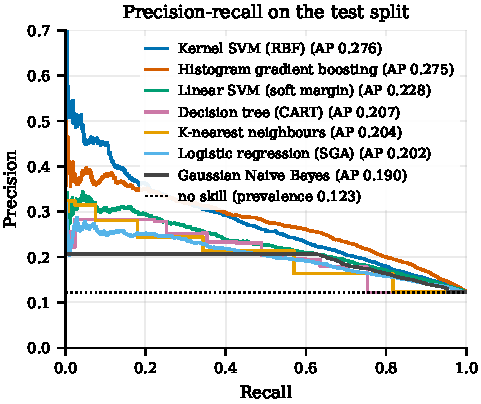
\includegraphics[width=\columnwidth]{fig1_pr_baselines.pdf}
  \caption{Precision-recall curves on the test split. The dotted line is the
  no-skill level, equal to the \num{0.1228} prevalence. The vertical axis is
  truncated at \num{0.70}: below a recall of about \num{0.02} the curves are
  decided by a handful of images and swing between \num{0} and \num{1}.}
  \label{fig:pr}
\end{figure}

\begin{figure}[t]
  \centering
  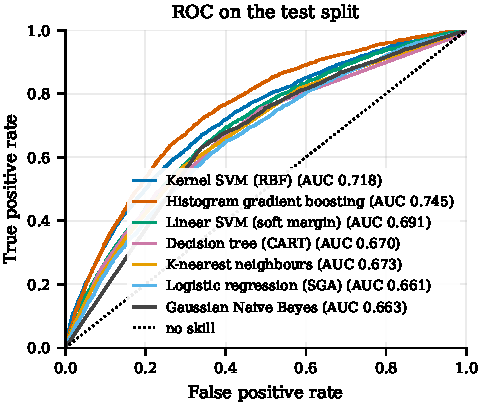
\includegraphics[width=\columnwidth]{fig2_roc_baselines.pdf}
  \caption{ROC curves for the same seven models and the same score vectors as
  \cref{fig:pr}. The two views do not agree on the ordering of the top two
  models, and the ROC view makes all seven look closer to one another than the
  precision-recall view does.}
  \label{fig:roc}
\end{figure}

Three observations deserve to be separated, because each is a different way the
imbalance distorts a familiar metric.

\paragraph{Accuracy ranks a constant classifier first.}
Six of the seven models sit between \num{0.8522} and \num{0.8772} test accuracy,
inside the band around the \num{0.8772} that an always-negative answer scores.
The highest accuracy of the table, \num{0.8772}, belongs to the RBF kernel
machine, and it is exactly that trivial value because at margin~\num{0} the
model makes \emph{no} positive call at all on the \num{22433} test images:
\num{0} true positives and \num{0} false positives. The model with the best test
average precision of the table is therefore also the one whose hard predictions
carry no information. Accuracy appears in \cref{tab:baselines} for completeness
and is used nowhere else in this work.

\paragraph{F1 at the default cut-off inverts the ranking.}
Gaussian naive Bayes has the second worst average precision (\num{0.1898} on
test) and the best default F1 (\num{0.2995}), while boosting has the best
average precision and an F1 of \num{0.0870}. The cause is visible in the number
of positive calls: naive Bayes issues \num{9681} of them on \num{22433} images,
against \num{348} for boosting and \num{0} for the RBF machine. Multiplying
\num{784} near-duplicate likelihood terms over strongly correlated pixels drives
the posterior to the ends of $[0,1]$, which leaves the default \num{0.5} cut-off
in a region where almost every image is called positive; the F1 maximising
threshold selected on validation for that model is \num{1.0000}, the boundary of
the interval, which is the signature of a saturated posterior. Naive Bayes is
not better at detecting effusion, it is differently miscalibrated. Any
conclusion drawn from F1 at the default threshold on this task would be an
artefact of calibration.

\paragraph{ROC and precision-recall disagree where it matters.}
Boosting dominates on ROC AUC (\num{0.7447} against \num{0.7175} for the RBF
machine) but the two are level on test average precision (\num{0.2753} against
\num{0.2763}). The reversal is the arithmetic of \cref{sec:protocol-metrics}:
the \num{19679} negative test images in the denominator of the false positive
rate absorb precisely the errors that the precision-recall view charges to the
model. \Cref{fig:roc} also compresses the seven models into a narrow band, which
would suggest that the choice of family hardly matters, whereas \cref{fig:pr}
separates boosting and the kernel machine from the rest over most of the recall
range. This is the concrete form, on this dataset, of the argument of Davis and
Goadrich~\cite{davis2006relationship} and of Saito and
Rehmsmeier~\cite{saito2015precision}.

One cost belongs next to the scores. The RBF machine needs \SI{146.7}{\second}
to score the \num{22433} test images against \SI{2.1}{\second} for boosting, a
factor of \num{69}, because its decision function is a sum over several thousand
support vectors in \num{784} dimensions. At equal average precision, boosting is
the better engineering choice.

\subsection{Where the decision boundary sits}
\label{sec:results-operating}

\Cref{tab:operating} reads the same seven models at a second operating point,
the threshold that maximises F1 on validation, transferred unchanged to test.
Every model improves and the degenerate cases disappear: boosting goes from
\num{0.0870} to \num{0.3639}, the RBF machine from \num{0.0000} to \num{0.3411},
the linear machine from \num{0.0610} to \num{0.3070}. Naive Bayes, first at the
default cut-off with \num{0.2995}, moves only to \num{0.3099} and falls back to
the middle of the table. The ordering by F1 at the selected threshold then
broadly follows the ordering by average precision, which is the expected
behaviour: once the threshold stops being an uncontrolled variable, the
thresholded metric measures the same underlying ranking quality.

\begin{table*}[t]
  \centering
  \caption{Test precision, recall and F1 at the default cut-off of each family
  (\num{0.5} on a posterior, \num{0} on a margin) and at the cut-off that
  maximises validation F1. The test split is never used to choose the threshold.
  Every model gains, and the two models that made almost no positive call at the
  default cut-off gain the most.}
  \label{tab:operating}
  \small
  \begin{tabular}{lcccccc}
\toprule
\multirow{2}{*}{Model} & \multicolumn{3}{c}{Default cut-off} & \multicolumn{3}{c}{Cut-off chosen on validation} \\
\cmidrule(lr){2-4}\cmidrule(l){5-7}
 & Prec. & Rec. & F1 & Prec. & Rec. & F1 \\
\midrule
Histogram gradient boosting & 0.388 & 0.049 & 0.087 & 0.264 & 0.587 & 0.364 \\
Kernel SVM (RBF) & 0.000 & 0.000 & 0.000 & 0.264 & 0.483 & 0.341 \\
Linear SVM (soft margin) & 0.317 & 0.034 & 0.061 & 0.235 & 0.442 & 0.307 \\
K-nearest neighbours & 0.324 & 0.024 & 0.045 & 0.213 & 0.570 & 0.310 \\
Decision tree (CART) & 0.244 & 0.016 & 0.029 & 0.231 & 0.490 & 0.314 \\
Gaussian Naive Bayes & 0.192 & 0.676 & 0.299 & 0.207 & 0.614 & 0.310 \\
Logistic regression (SGA) & 0.250 & 0.102 & 0.145 & 0.205 & 0.484 & 0.288 \\
\bottomrule
\end{tabular}

\end{table*}

\begin{figure}[t]
  \centering
  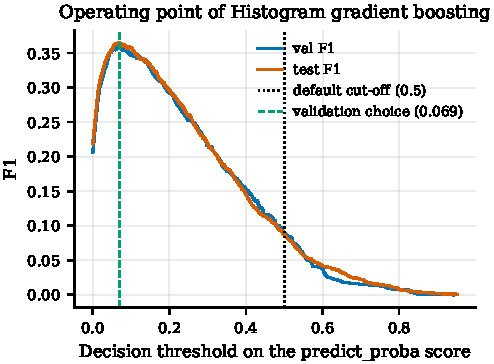
\includegraphics[width=\columnwidth]{fig5_threshold_sensitivity.pdf}
  \caption{F1 of the boosted model against its decision threshold, on validation
  and on test. The default \num{0.5} cut-off lies far to the right of the
  maximum, which on this prevalence sits near \num{0.07}. The two curves peak at
  nearly the same place, so the threshold transfers across splits.}
  \label{fig:threshold}
\end{figure}

\Cref{fig:threshold} shows why. For the boosted model the F1 maximum lies at a
posterior of \num{0.0691}, not at \num{0.5}, and the validation and test curves
peak at nearly the same place, so the choice transfers. The practical reading is
that a thresholded metric on an imbalanced task reports the sum of two things,
the quality of the ranking and the accident of where the library put the
cut-off, and that the second term dominates here. This is why average precision
drives every selection decision in this work, and why \cref{tab:robustness}
reports F1 at the validation selected point rather than at the default one.

\subsection{Does reducing the dimension help?}
\label{sec:results-representation}

The two families whose behaviour depends most directly on the ambient dimension
were rerun on a \num{50} component principal projection fitted on the training
subsample, retaining \num{95.3} percent of the variance
(\cref{tab:representation}). Neither improves. The $K=5$ neighbours rule falls
from \num{0.1822} to \num{0.1776} validation average precision and the RBF
machine from \num{0.2417} to \num{0.2344}. The expectation behind the ablation,
that Euclidean distances and an isotropic kernel would behave better once
\num{784} correlated pixel coordinates are compressed, is not met. The
discriminative signal lies partly in directions that principal component
analysis discards for carrying little variance, which is plausible on this
modality: variance in a chest radiograph is dominated by patient size, framing
and exposure, none of which is the costophrenic angle. The projection does buy
computation, since the RBF machine then scores the test split in
\SI{21.9}{\second} instead of \SI{146.7}{\second}, a factor of \num{6.7}, for
\num{0.008} of average precision. That trade is worth taking in deployment and
not worth taking when the point is to compare model families, so the main tables
keep the \num{784} dimensional features.

\begin{table}[t]
  \centering
  \caption{Representation check on the primary seed. The principal basis is
  fitted on the training subsample only and retains \num{95.3} percent of the
  variance.}
  \label{tab:representation}
  \footnotesize\setlength{\tabcolsep}{4pt}
  \begin{tabular}{lcccc}
\toprule
\multirow{2}{*}{Model} & \multicolumn{2}{c}{Pixels (784)} & \multicolumn{2}{c}{PCA (50)} \\
\cmidrule(lr){2-3}\cmidrule(l){4-5}
 & AUC & AP & AUC & AP \\
\midrule
KNN, $K = 5$ & 0.6336 & 0.1819 & 0.6317 & 0.1810 \\
Kernel SVM, $C = 1$ & 0.7175 & 0.2763 & 0.7086 & 0.2683 \\
\bottomrule
\end{tabular}

\end{table}

% =====================================================================
%  TP4, Phase III, closing discussion: what the experiment does not settle,
%  and the handover to the evidential modelling of Phase IV.
%  Author: FOMETHE SOBMBANANG MAXIMILIEN
%  Fragment, included by phase3_sections.tex. It continues the section
%  opened by phase3_results.tex.
% =====================================================================

\subsection{What these experiments do not settle}
\label{sec:results-limits}

Four limits bound every claim made above, and they are stated here rather than
left for a reader to infer.

\paragraph{The images are thumbnails and the features are pixels.}
A pleural effusion is read on a radiograph as blunting of the costophrenic angle
and a fluid meniscus at the lung base, a local geometric cue occupying a small
part of the image. At \num{28}\,$\times$\,\num{28} that region covers a few
pixels, and a flat vector of \num{784} intensities gives none of the models any
notion of adjacency. The absolute scores reported here should be read as what
classical classifiers extract from a thumbnail, not as an estimate of what is
achievable on full resolution radiographs. The comparison that this work
supports is the one between families, conditions and metrics, all measured under
one fixed representation.

\paragraph{Published numbers are not directly comparable.}
The MedMNIST authors report a convolutional baseline on the same
\num{28}\,$\times$\,\num{28} ChestMNIST images~\cite{yang2023medmnist}, but
averaged over the \num{14} findings and as area under the ROC curve, whereas
this study reports a single finding and relies on average precision. A
difference in target, in metric and in the number of training images is enough
to make a direct ranking meaningless. Published figures and the figures of this
work are therefore kept in separate tables, and no claim of superiority or
inferiority is made across them.

\paragraph{The clean condition is not a clean reference.}
The annotations of ChestX-ray14, which ChestMNIST
redistributes~\cite{wang2017chestxray8}, were extracted from free-text
radiology reports by natural language processing rather than assigned by a
reader looking at the image. They therefore carry an error rate of their own,
unknown and not measurable from the data at hand. The condition called
\emph{clean} in \cref{tab:robustness} is the published annotation, not ground
truth, so the \num{5} percent corruption of Task~3.2 is an increment on top of a
baseline error whose size is not known. Any true degradation curve is shifted
along an axis whose origin is not observed, which compresses the effect that the
experiment can see.

\paragraph{One corruption model, one rate, one direction.}
The simulation flips a fixed fraction of the positive training labels to
negative, independently of the image content. Real annotation error is not
independent of the image: a faint effusion is missed more often than a large
one, which makes the noise instance dependent and concentrated near the decision
boundary, exactly where it is most harmful. The experiment also uses a single
rate and a single target finding. Results obtained under class-conditional noise
at \num{5} percent do not transfer by themselves to instance-dependent noise, to
higher rates, or to the other thirteen findings. Finally, ChestMNIST has no
explicit uncertainty category, unlike CheXpert~\cite{irvin2019chexpert}, whose
reports distinguish an uncertain mention from a negative one; the uncertainty
studied here is simulated for that reason, which is also the gap that Phase~IV
addresses with a model that represents it directly.

Two smaller points belong in the same list. Model selection uses a single
validation split rather than cross-validation, so the selection itself carries a
variance that is not quantified. And the posteriors are used only for ranking:
no calibration measure is reported, although \cref{sec:results-baselines} shows
at least one model, Gaussian naive Bayes, whose posterior is badly enough
calibrated to change which metric ranks it first.

\subsection{From constraining a model to representing evidence}
\label{sec:results-bridge}

The robustness mechanism tested in this phase is the only one classical
regularisation offers: shrink the hypothesis class so that a handful of wrong
labels cannot move the boundary far. It acts on the whole function, uniformly,
before any particular image is seen. It gives the model no way of behaving
differently on an image that resembles its training data and on one that does
not.

That limitation is visible in the outputs these models produce. A sigmoid
posterior of \num{0.5} is returned both for a radiograph that genuinely lies
between the two classes, where the evidence is balanced, and for a radiograph
unlike anything in the training set, where there is no evidence at all. The two
situations are clinically opposite and numerically identical, and no choice of
$\lambda$, of $C$ or of tree depth separates them, because a point estimate of a
probability has no room to carry that distinction. The operating point analysis
of \cref{sec:results-operating} makes the same point from another side: the
number the model emits is a score to be ranked, and the meaning attached to its
value is supplied from outside, by a threshold chosen on validation.

This is the opening that evidential deep learning fills. Rather than emitting a
probability, such a model emits the parameters of a Dirichlet distribution over
the class probabilities, so that the amount of evidence accumulated for an image
and the belief left uncommitted become explicit outputs alongside the
prediction~\cite{sensoy2018evidential}. The empirical ground established here,
that constraining capacity leaves the degradation under label noise of the same
order as the seed-to-seed variability, is what motivates looking for robustness
in the output representation rather than only in the size of the hypothesis
class. The formal treatment of that argument belongs to Phase~IV.



\bibliographystyle{plain}
\bibliography{references_phase3}

\end{document}
